\chapter{Experiments}\label{chap:experiments}

% 
% \begin{figure}[t]
% \begin{centering}
%     \subfloat[Some cool graphic]
%     {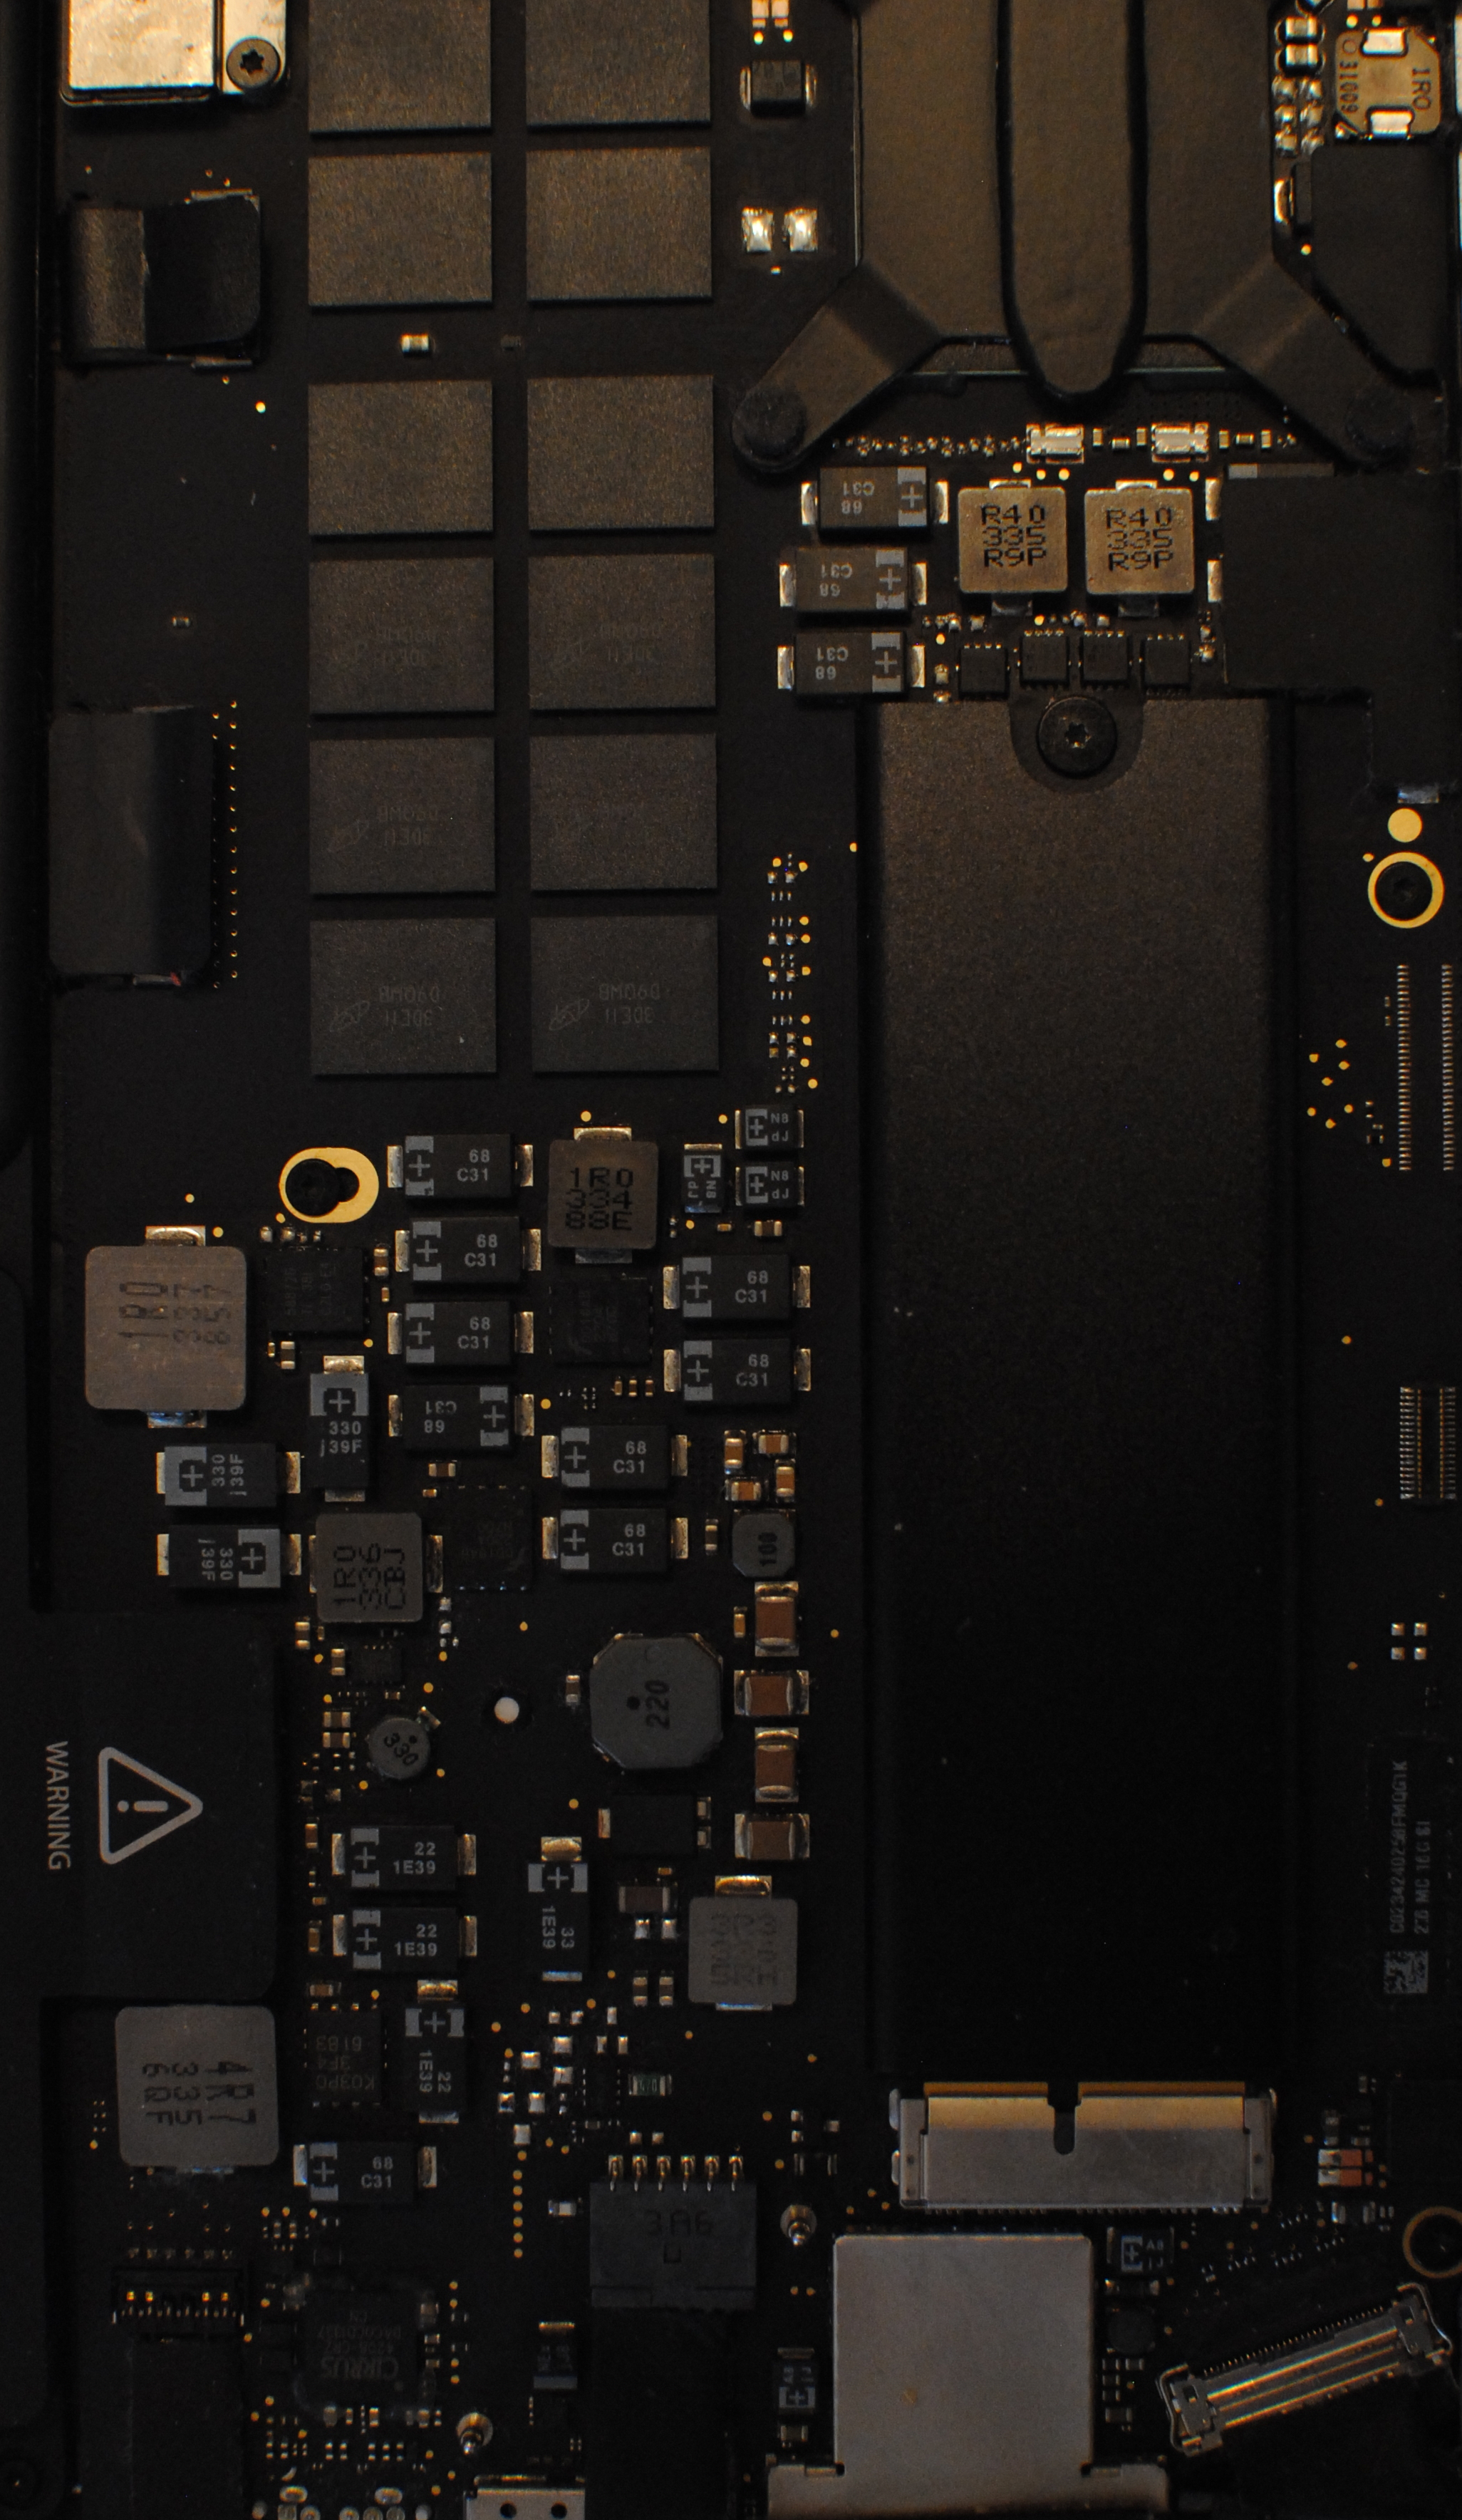
\includegraphics[scale=0.2]{figures/experiments/img.JPG}}
%
%     \subfloat[Some cool related graphic]
%     {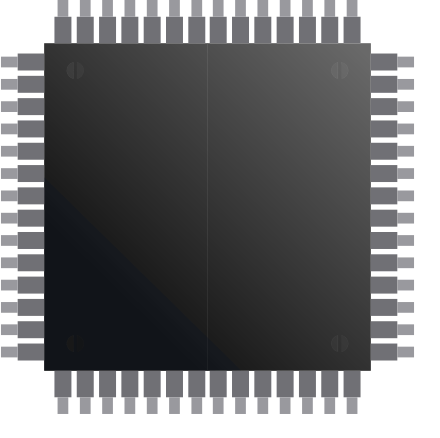
\includegraphics[scale=0.4]{figures/experiments/microcontroller.png}}
%     \caption[Caption that appears in the figlist]{\textbf{Caption that appears under the fig} \lipsum[1-1]}
%     \label{fig:pcaclasses}
% \end{centering}
% \end{figure}

% \begin{table}[ht]
\centering
% spacing in table
\ra{1.3}
\begin{tabular}{@{}lr@{}}
  \toprule
  Type & Accuracy\\ \midrule
  A    & 82.47 $\pm$ 3.21 \\
  B    & 78.47 $\pm$ 2.43 \\
  C    & 84.30 $\pm$ 2.35 \\
  D    & 86.81 $\pm$ 3.01 \\
  \bottomrule
\end{tabular}

    \caption[Table caption]{\textbf{Table caption.} foo bar...\\}
    \label{tab:accuracy}
\end{table}


times (precomputed correction factors):
\begin{verbatim}
542.32user 447.26system 16:26.02elapsed 100\%CPU (0avgtext+0avgdata 116107220maxresident)k
14528inputs+8outputs (20major+159388812minor)pagefaults 0swaps
\end{verbatim}

But for which setup? single-core? the small\_test\_matrix?


% Experiments
\todo{The time-resource-measures done}


